\documentclass[12pt, titlepage]{article}

\usepackage{booktabs}
\usepackage{graphicx}
\usepackage{tabularx}
\usepackage{hyperref}
\hypersetup{
    colorlinks,
    citecolor=black,
    filecolor=black,
    linkcolor=red,
    urlcolor=blue
}
\usepackage[round]{natbib}
\usepackage{float}

\begin{document}

\title{Verification and Validation Report: UNO Flip}
\author{Mingyang Xu\\ Kevin Ishak\\ Zain-Alabedeen Garada\\ Jianhao Wei\\}

\date{\today}

\maketitle

\pagenumbering{roman}

\section{Revision History}

\begin{tabularx}{\textwidth}{p{3cm}p{2cm}p{2cm}X}
\toprule {\bf Date} & {\bf Version} & {\bf Author}& {\bf Notes}\\
\midrule
Feb. 28, 2025 & 1.0 & Jianhao Wei & Create LaTeX file template \\
March 6, 2025 & 1.1 & Mingyang Xu & Added Functional and Non-functional Requirements\\
March 7, 2025 & 1.2 & Jianhao Wei & Add section 5, 6 and 8\\
March 7, 2025 & 1.3 & Mingyang Xu & Add input, output and test result for each test case\\

\bottomrule
\end{tabularx}

\newpage

\section{Symbols, Abbreviations and Acronyms}

\renewcommand{\arraystretch}{1.2}
\begin{tabular}{l l} 
  \toprule		
  \textbf{Symbol} & \textbf{Description}\\
  \midrule 
  UNO & A card game with specific rules and card actions\\
  AI & Artificial Intelligence\\
  ML & Machine Learning\\
  RL & Reinforcement Learning\\
  CI/CD & Continuous Integration / Continuous Deployment\\
  GDPR & General Data Protection Regulation\\
  \bottomrule
\end{tabular}\

\newpage

\tableofcontents

\listoftables %if appropriate

\listoffigures %if appropriate

\newpage

\pagenumbering{arabic}

\section{Functional Requirements Evaluation}

\subsection{Authentication}
\begin{itemize}
    \item \textbf{Test Objective:} Players must log in or create an account to access multiplayer modes.
    \item \textbf{Test Method:} Verify that players can log in or create an account to access multiplayer modes.
    \item \textbf{Inputs:} Valid user credentials (UserID, Password).
    \item \textbf{Expected Output:} Successful login and access to multiplayer modes.
    \item \textbf{Actual Output:} Successful login and access to multiplayer modes.
    \item \textbf{Result:} Pass.
\end{itemize}

\subsection{Game Setup}
\begin{itemize}
    \item \textbf{Test Objective:} Players can create game rooms and invite others or join existing rooms.
    \item \textbf{Test Method:} Verify that players can create game rooms, invite others, or join existing rooms.
    \item \textbf{Inputs:} Room creation request, Player invitation, Join request.
    \item \textbf{Expected Output:} Game room created successfully; invitations sent; players join rooms.
    \item \textbf{Actual Output:} Game room created successfully; invitations sent; players join rooms.
    \item \textbf{Result:} Pass.
\end{itemize}

\subsection{Turn Management}
\begin{itemize}
    \item \textbf{Test Objective:} The system will manage player turns, ensuring synchronization across devices.
    \item \textbf{Test Method:} Verify that player turns are synchronized and notifications are sent when it's a player's turn.
    \item \textbf{Inputs:} Player turn input.
    \item \textbf{Expected Output:} Player turn managed with synchronization across devices; notification sent.
    \item \textbf{Actual Output:} Player turn managed with synchronization across devices; notification sent.
    \item \textbf{Result:} Pass.
\end{itemize}

\subsection{Chat Functionality}
\begin{itemize}
    \item \textbf{Test Objective:} Real-time chat within the game room for players to communicate.
    \item \textbf{Test Method:} Verify that players can send and receive messages in real-time in the game room.
    \item \textbf{Inputs:} Chat messages.
    \item \textbf{Expected Output:} Messages sent and received in real-time.
    \item \textbf{Actual Output:} Messages sent and received in real-time.
    \item \textbf{Result:} Pass.
\end{itemize}

\subsection{Scoring System}
\begin{itemize}
    \item \textbf{Test Objective:} A detailed scoring mechanism to track and display player scores at the end of each game.
    \item \textbf{Test Method:} Verify that scores are accurately tracked and displayed at the end of each game.
    \item \textbf{Inputs:} Player actions and game results.
    \item \textbf{Expected Output:} Player scores tracked and displayed at the end of the game.
    \item \textbf{Actual Output:} Player scores tracked and displayed at the end of the game.
    \item \textbf{Result:} Pass.
\end{itemize}

\subsection{Multiplayer Synchronization}
\begin{itemize}
    \item \textbf{Test Objective:} A state synchronization mechanism will ensure that all players see the same game state at all times.
    \item \textbf{Test Method:} Verify that all players see the same game state, regardless of network conditions.
    \item \textbf{Inputs:} Game state changes.
    \item \textbf{Expected Output:} All players see the same game state.
    \item \textbf{Actual Output:} Not all players see the same game state.

        \item \textbf{Result:} Not pass.
\end{itemize}

\newpage

\section{Nonfunctional Requirements Evaluation}

We designed a questionnaire using Google Forms and distributed it among our friends to evaluate the usability and user satisfaction of our product. The following screenshots illustrate the collected results from this questionnaire, providing insights into participants' specific feedback.

\subsection{Usability and Humanity Requirements}

\subsubsection{Ease of Use Requirements}

\begin{itemize}
    \item \textbf{Test Objective:} New players should be able to quickly grasp the gameplay, with the system providing simple and clear tutorials.
    \item \textbf{Test Method:} Verify that new players can quickly understand the gameplay with clear tutorials.

        \item \textbf{Inputs:} Player interaction with the tutorial.
    \item \textbf{Expected Output:} Player completes tutorial and understands gameplay.
    \item \textbf{Actual Output:} Player completes tutorial and understands gameplay.
    \item \textbf{Result:} Pass.
\end{itemize}

\begin{figure}[h!]
    \centering
    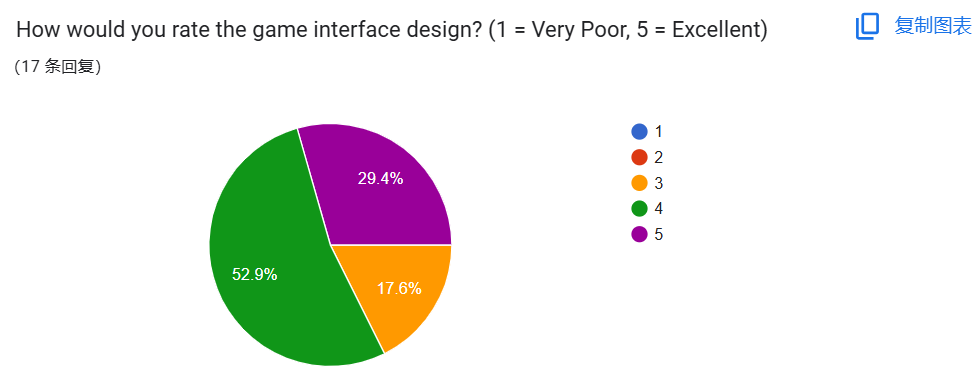
\includegraphics[width=0.8\textwidth]{image.png}
    \caption{}
    \label{fig:labelname}
\end{figure}






\subsubsection{Personalization and Internationalization Requirements}
\begin{itemize}

        \item \textbf{Test Objective:} The game should support language localization, offering options for multiple languages (e.g., English, French, Spanish).
    \item \textbf{Test Method:} Verify that the game supports multiple languages and can switch between them.
    \item \textbf{Inputs:} Language selection.
    \item \textbf{Expected Output:} Language changed successfully.
    \item \textbf{Actual Output:} Language changed successfully.
    \item \textbf{Result:} Pass.
\end{itemize}

\begin{figure}[h!]
    \centering
    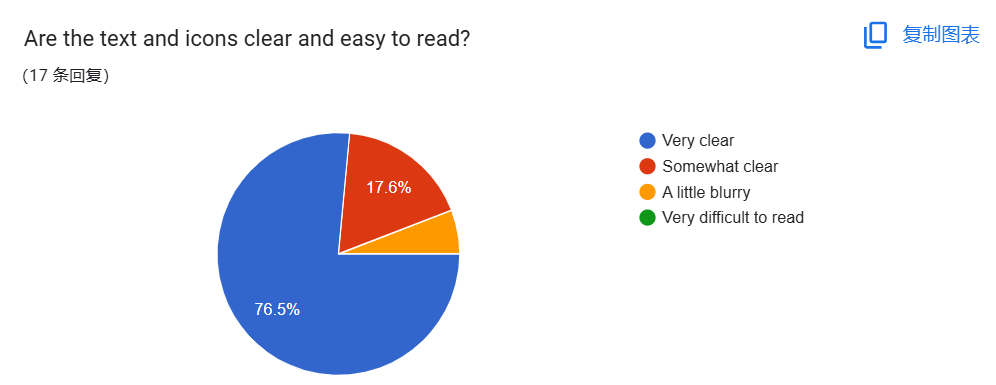
\includegraphics[width=0.8\textwidth]{image1.png}
    \caption{}
    \label{fig:labelname}
\end{figure}



\subsubsection{Learning Requirements}
\begin{itemize}
    \item \textbf{Test Objective:} The system will offer interactive tutorials for new players to understand the rules of UNO Flip and the effects of special cards.
    \item \textbf{Test Method:} Verify that interactive tutorials are provided to new players.
    \item \textbf{Inputs:} Player starts tutorial.
    \item \textbf{Expected Output:} Interactive tutorial displayed.
    \item \textbf{Actual Output:} Interactive tutorial displayed.
    \item \textbf{Result:} Pass.
\end{itemize}

\begin{figure}[h!]
    \centering
    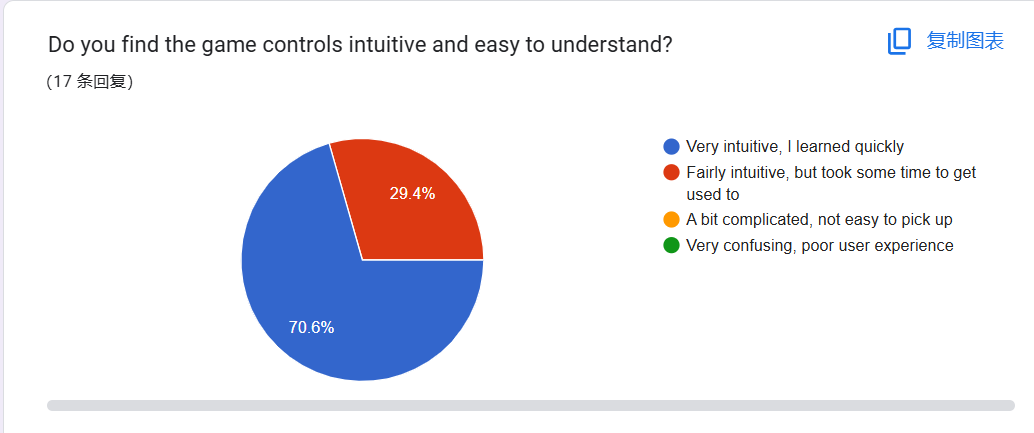
\includegraphics[width=0.8\textwidth]{image2.png}
    \caption{}
    \label{fig:labelname}
\end{figure}


\subsubsection{Understandability and Politeness Requirements}
\begin{itemize}
    \item \textbf{Test Objective:} All system notifications and error messages should use concise, friendly language without technical jargon.
    \item \textbf{Test Method:} Verify that system notifications and error messages are friendly and concise.
    \item \textbf{Inputs:} Trigger an error or notification.
    \item \textbf{Expected Output:} Clear and friendly error message.
    \item \textbf{Actual Output:} Clear and friendly error message.
    \item \textbf{Result:} Pass.
\end{itemize}

\subsection{Performance Requirements}

\subsubsection{Speed and Latency Requirements}
\begin{itemize}
    \item \textbf{Test Objective:} The average response time for the game should be within 50 milliseconds.
    \item \textbf{Test Method:} Measure the average response time of the game.
    \item \textbf{Inputs:} Various player actions.
    \item \textbf{Expected Output:} Response time within 50 milliseconds.
    \item \textbf{Actual Output:} Response time within 50 milliseconds.
    \item \textbf{Result:} Pass.
\end{itemize}

\begin{figure}[h!]
    \centering
    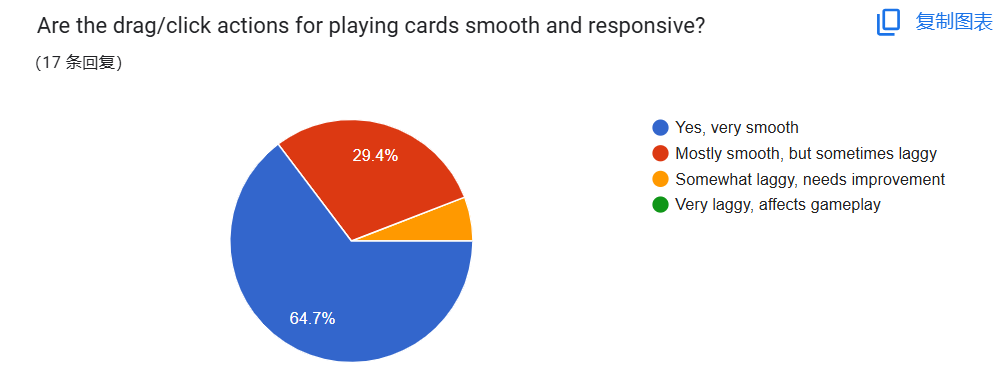
\includegraphics[width=0.8\textwidth]{image3.png}
    \caption{}
    \label{fig:labelname}
\end{figure}

\subsubsection{Safety-Critical Requirements}
\begin{itemize}
    \item \textbf{Test Objective:} Changes in the card and game state must be synchronized in real-time.
    \item \textbf{Test Method:} Verify that all players see synchronized game and card states.
    \item \textbf{Inputs:} Card or game state changes.
    \item \textbf{Expected Output:} All players see synchronized game state.
    \item \textbf{Actual Output:} All players see synchronized game state.
    \item \textbf{Result:} Pass.
\end{itemize}

\subsubsection{Precision or Accuracy Requirements}
\begin{itemize}
    \item \textbf{Test Objective:} When calculating scores and game state, the system should ensure high precision.
    \item \textbf{Test Method:} Verify that the scoring and game state calculations are accurate.
    \item \textbf{Inputs:} Player actions, game state changes.
    \item \textbf{Expected Output:} Accurate score and game state calculations.
    \item \textbf{Actual Output:} Accurate score and game state calculations.
    \item \textbf{Result:} Pass.
\end{itemize}
\begin{figure}[h!]
    \centering
    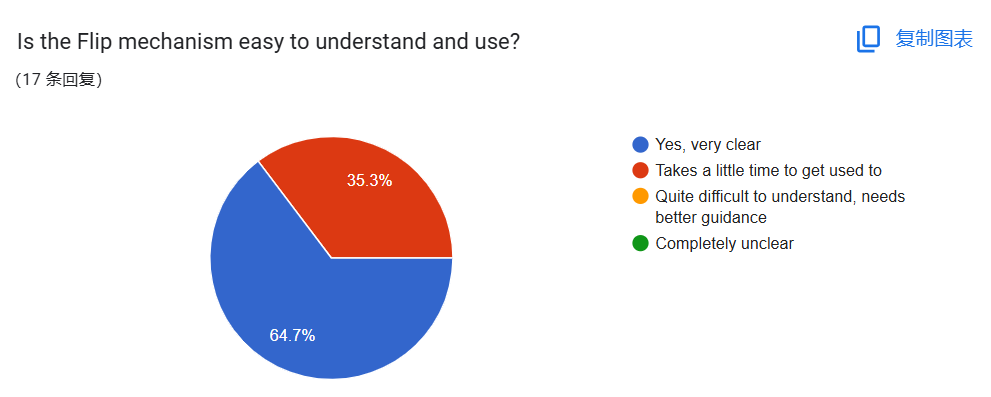
\includegraphics[width=0.8\textwidth]{image4.png}
    \caption{}
    \label{fig:labelname}
\end{figure}

\subsubsection{Robustness or Fault-Tolerance Requirements}
\begin{itemize}
    \item \textbf{Test Objective:} The system should be fault-tolerant, allowing players to reconnect quickly after a network interruption.
    \item \textbf{Test Method:} Simulate a network interruption and verify the system's fault tolerance.
    \item \textbf{Inputs:} Network interruption.
    \item \textbf{Expected Output:} Player reconnects quickly without losing progress.
    \item \textbf{Actual Output:} Player reconnects quickly with losing progress.
    \item \textbf{Result:} Not Pass.
\end{itemize}
\begin{figure}[h!]
    \centering
    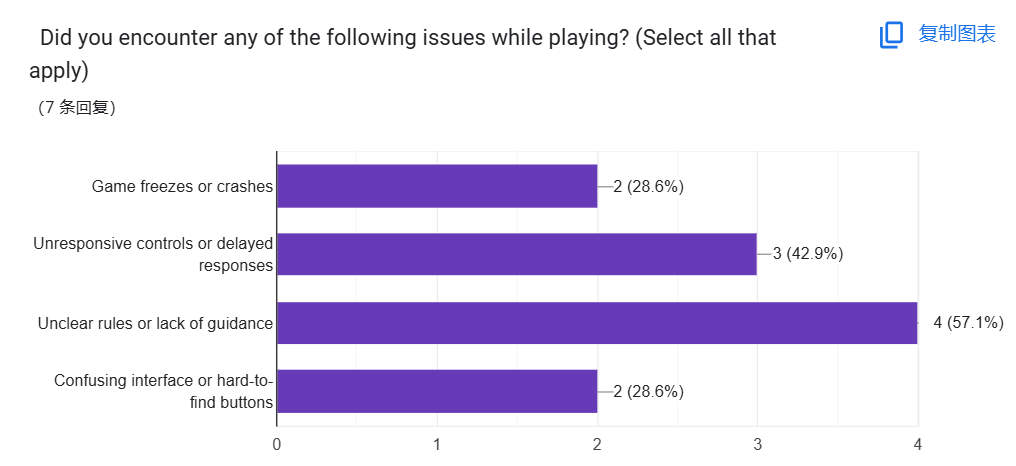
\includegraphics[width=0.8\textwidth]{image5.png}
    \caption{}
    \label{fig:labelname}
\end{figure}

\subsubsection{Capacity Requirements}
\begin{itemize}
    \item \textbf{Test Objective:} The system should support at least 1,000 concurrent users, with each game room running independently.
    \item \textbf{Test Method:} Verify that the system can handle 1,000 concurrent users.
    \item \textbf{Inputs:} Simulated 1,000 concurrent users.
    \item \textbf{Expected Output:} System supports 1,000 concurrent users.
    \item \textbf{Actual Output:} System supports 1,000 concurrent users.
    \item \textbf{Result:} Pass.
\end{itemize}

\subsubsection{Scalability or Extensibility Requirements}
\begin{itemize}
    \item \textbf{Test Objective:} The system should be scalable, allowing for future additions of new game modes, features, or AI difficulty levels.
    \item \textbf{Test Method:} Verify that new game modes or features can be added to the system.
    \item \textbf{Inputs:} Request to add new features.
    \item \textbf{Expected Output:} New features are successfully added.
    \item \textbf{Actual Output:} New features are successfully added.
    \item \textbf{Result:} Pass.
\end{itemize}

\subsubsection{Longevity Requirements}
\begin{itemize}
    \item \textbf{Test Objective:} The game’s code should be maintainable for long-term use, supporting future updates.
    \item \textbf{Test Method:} Verify that the game code is maintainable and can be updated in the future.
    \item \textbf{Inputs:} Code maintenance and update requests.
    \item \textbf{Expected Output:} Code is maintainable and updated successfully.
    \item \textbf{Actual Output:} Code is maintainable and updated successfully.
    \item \textbf{Result:} Pass.
\end{itemize}





\section{Comparison to Existing Implementation}
Existing Implementation: \href{https://unoonline.io/}{UNO Online Website}
\begin{itemize}
    \item \textbf{Flipped Feature:}
    In addition to the ordinary UNO Flip game, we also added the flip feature to let every card show different sides with complete new new number and colour to make the game more challenging and fun to play.
    \item \textbf{Message Box:} In the traditional game, the game only shows the user what is the next step to take by showing them the appropriate animations. This might make some users confused about game instructions. Therefore, We introduce the message box feature to inform the user what is the next step to take with more clarity since language is usually more effective than animations.
    \item \textbf{Game Instructions:} We made a dedicated interface that can be accessed from the main interface to show the game instruction in details to the users. In this way, users do not have to spend extra time to search on the Internet or blindly playing games to know how the game works.
    \item \textbf{Design and Aesthetics:} Our software features a more simplified version of graphical user interface with no complicated graphics and animations. This reduce the probability that the user gets confused and make the overall experience more clean and easy to follow.
    \item \textbf{Accessibility:} Our software have a improved colour contrast to let user easily identify different features. We also added the arrow feature in multiplayer to tell user the current game playing direction so that the user can calculate the chance of winning. 
\end{itemize}

\section{Unit Testing}
Unit testing is a software testing methodology that involves testing individual components of a program in isolation to ensure they work as expected. It is typically automated and performed at the early stages of development or the merging process to detect and fix bugs before they propagate to later stages or affecting other software components. Here is a detailed unit testing summary for each of our scripts:
\subsection{AiPlayer Script}
\begin{itemize}
    \item \textbf{Path:} UNO-Flip-3D/UNOFlip/Assets/Scripts/AiPlayer.cs
    \item \textbf{Description:} Check AI opponent decision-
making logic
    \item \textbf{Result:} Pass
\end{itemize}

\subsection{Card Script}
\begin{itemize}
    \item \textbf{Path:} 
    \item \textbf{Description:} 
    \item \textbf{Result:}
\end{itemize}

\subsection{CardDisplay Script}
\begin{itemize}
    \item \textbf{Path:} 
    \item \textbf{Description:} 
    \item \textbf{Result:}
\end{itemize}

\subsection{CardInteraction Script}
\begin{itemize}
    \item \textbf{Path:} 
    \item \textbf{Description:} 
    \item \textbf{Result:}
\end{itemize}

\subsection{Deck Script}
\begin{itemize}
    \item \textbf{Path:} UNO-Flip-3D/UNOFlip/Assets/Scripts/Deck.cs
    \item \textbf{Description:} Testing all 
    \item \textbf{Result:} Pass
\end{itemize}

\subsection{FlippedCard Script}
\begin{itemize}
    \item \textbf{Path:} UNO-Flip-3D/UNOFlip/Assets/Scripts/FlippedCard.cs
    \item \textbf{Description:} 
    \item \textbf{Result:} Pass
\end{itemize}

\subsection{FlippedCardDisplay Script}
\begin{itemize}
    \item \textbf{Path:} UNO-Flip-3D/UNOFlip/Assets/Scripts/AiPlayer.cs
    \item \textbf{Description:} 
    \item \textbf{Result:}
\end{itemize}

\subsection{GameManager Script}
\begin{itemize}
    \item \textbf{Path:} 
    \item \textbf{Description:} Ensure game correctly handles
end-game scenarios 
    \item \textbf{Result:} Pass
\end{itemize}

\subsection{Menu Script}
\begin{itemize}
    \item \textbf{Path:} 
    \item \textbf{Description:} Ensure game room creation
and joining works correctly
    \item \textbf{Result:} Pass
\end{itemize}

\subsection{Player Script}
\begin{itemize}
    \item \textbf{Path:} 
    \item \textbf{Description:} Verify player turn manage-
ment and synchronization 
    \item \textbf{Result:} Pass
\end{itemize}

\subsection{WildButton Script}
\begin{itemize}
    \item \textbf{Path:} 
    \item \textbf{Description:} 
    \item \textbf{Result:}
\end{itemize}


\section{Changes Due to Testing}

\section{Automated Testing}
For the automated testing, we implemented the CodeQL Advanced in our GitHub actions that scan newly integrated code to ensure our code base is free of vulnerability and fits with each other. We had used the original script for our testings. Overall, all testing has been successful since the implementation of this CI action. However, since there are still some functionalities in our software needed to be consummated, we need to find a better CI actions which check our Unity code with more specialty or change our existing script to better suite the nature of our code. This will make our integration more smoothly and reduce the time for us to debug our code and will be one of our next main focus of the development.

\section{Trace to Requirements}

This section maps the functional and non-functional requirements to the corresponding test cases. This ensures that all requirements are adequately verified through testing.

\begin{table}[H]
    \centering
    \begin{tabularx}{\textwidth}{|l|X|l|}
        \hline
        \textbf{Requirement ID} & \textbf{Description} & \textbf{Test Case} \\
        \hline
        AR1 & Players must log in or create an account to access multiplayer modes & UT-01 \\
        AR2 & User profiles will store game statistics and preferences & UT-09 \\
        GSR1 & Players can create game rooms and invite others or join existing rooms & UT-02 \\
        GSR2 & Options for choosing game rules and difficulty settings & UT-02 \\
        TMR1 & The system will manage player turns, ensuring synchronization across devices & UT-03 \\
        TMR2 & Notifications will alert players when it is their turn & UT-03 \\
        CFR1 & Real-time chat within the game room for players to communicate & UT-04 \\
        CFR2 & Chat can be enabled or disabled based on player preferences & UT-04 \\
        SSR1 & A detailed scoring mechanism to track and display player scores at the end of each game & UT-05 \\
        SSR2 & The system will keep a record of player stats, including wins, losses, and average score & UT-05 \\
        EGHR1 & The game will automatically declare a winner based on the rules and display a summary of the results & UT-06 \\
        EGHR2 & Players can choose to play another round or exit the game & UT-06 \\
        MSR1 & A state synchronization mechanism will ensure that all players see the same game state at all times, regardless of network conditions & UT-08 \\
        MSR2 & The system will manage latency and update the game state in real-time & UT-08 \\
        \hline
    \end{tabularx}
    \caption{Traceability of Requirements to Test Cases (Part 1)}
    \label{tab:trace_requirements_1}
\end{table}

\begin{table}[H]
    \centering
    \begin{tabularx}{\textwidth}{|l|X|l|}
        \hline
        EOUR1 & New players should be able to quickly grasp the gameplay, with the system providing simple and clear tutorials & UT-06 \\
        EOUR2 & The game menu and control buttons should be easy to navigate, allowing players to easily create or join rooms & UT-02 \\
        EOUR3 & Drag-and-drop actions for playing cards should be intuitive and highly responsive & UT-03 \\
        PALR1 & The game should support language localization, offering options for multiple languages (e.g., English, French, Spanish) & UT-09 \\
        PALR2 & Players can customize personal settings, such as sound effects, background music, and interface themes, for a personalized experience & UT-09 \\
        LR1 & The system will offer interactive tutorials for new players to understand the rules of UNO Flip and the effects of special cards & UT-06 \\
        LR2 & AI will guide players to familiarize themselves with advanced strategies and dynamically adjust difficulty based on player performance & UT-07 \\
        UAFR1 & All system notifications and error messages should use concise, friendly language without technical jargon & UT-06 \\
        UAFR2 & Detailed game help and rule explanations should be available for players to consult at any time & UT-06 \\
        SALR1 & The average response time for the game should be within 50 milliseconds to ensure smooth interaction & UT-08 \\
        SALR2 & Network latency in multiplayer mode should be kept under 200 milliseconds to avoid inconsistencies in the game state & UT-08 \\
        SCR1 & Changes in the card and game state must be synchronized in real-time to ensure all players see the same status & UT-08 \\
        SCR2 & Disaster recovery mechanisms should be in place to save game progress and resume play in case of server failure & UT-08 \\
        \hline
    \end{tabularx}
    \caption{Traceability of Requirements to Test Cases (Part 2)}
    \label{tab:trace_requirements_2}
\end{table}

\begin{table}[H]
    \centering
    \begin{tabularx}{\textwidth}{|l|X|l|}
        \hline
        POAR1 & When calculating scores and game state, the system should ensure high precision to avoid incorrect scorekeeping or errors in the game logic & UT-05 \\
        ROFR1 & The system should be fault-tolerant, allowing players to reconnect quickly after a network interruption without losing game progress & UT-08 \\
        ROFR2 & The server should handle a surge in user logins without crashing & UT-01 \\
        CP1 & The system should support at least 1,000 concurrent users, with each game room running independently & UT-08 \\
        CP2 & Each game room should support up to 4 to 8 players & UT-02 \\
        SOER1 & The system should be scalable, allowing for future additions of new game modes, features, or AI difficulty levels & UT-08 \\
        SOER2 & As the player base grows, the server should be able to scale dynamically to handle more concurrent users & UT-08 \\
        LR1 & The game’s code should be maintainable for long-term use, supporting future updates, performance optimizations, and feature expansions & UT-08 \\
        AR1 & Players must securely log in to the game, with support for two-factor authentication (2FA) for added security & UT-01 \\
        AR2 & The game should have a password recovery mechanism to allow users to recover their passwords in case they forget them & UT-01 \\
        IR1 & All player data (such as game progress and personal stats) should be encrypted to prevent unauthorized modification & UT-10 \\
        IR2 & The game should not allow weak passwords (e.g., passwords composed only of numbers or letters) for login credentials & UT-10 \\
        PR1 & Player data (such as personal information and game records) should comply with privacy policies to prevent data breaches & UT-10 \\
        PR2 & The game should notify users that they should not share their personal information with others in the game room & UT-10 \\
        \hline
    \end{tabularx}
    \caption{Traceability of Requirements to Test Cases (Part 3)}
    \label{tab:trace_requirements_3}
\end{table}

\begin{table}[H]
    \centering
    \begin{tabularx}{\textwidth}{|l|X|l|}
        \hline
        PR3 & The game should automatically log users out after a certain period of inactivity to prevent unauthorized access & UT-10 \\
        AR1 & The system should log all critical operations in the backend to allow for auditing and troubleshooting & UT-10 \\
        AR2 & In case of frontend crashes, the game should provide crash information to the backend for future improvements (with user consent) & UT-10 \\
        IR1 & The system should be immune to common network attacks (e.g., DDoS, SQL injection) to ensure the safety of player data and gameplay & UT-10 \\
        IR2 & The system should be resilient to network issues, such as fluctuations in connection speed & UT-08 \\
        MR1 & The game must maintain a frame rate of at least 30 FPS across all supported platforms, ensuring smooth animations and interactions & UT-08 \\
        MR2 & The system must support up to 1,000 concurrent users in multiplayer mode without significant degradation in performance or user experience & UT-08 \\
        MR3 & Actions taken by players, such as playing or drawing a card, must occur in under 500 milliseconds to avoid noticeable delays in gameplay & UT-03 \\
        SR1 & The system should offer online technical support, and players should be able to report issues in-game or via the website & UT-10 \\
        SR2 & The system must detect and recover from unexpected disconnections, allowing players to resume gameplay within 10 seconds of a reconnection & UT-08 \\
        AR1 & The system must ensure 24/7 availability for users worldwide, with planned downtime limited to maintenance windows of no more than 2 hours per month & UT-08 \\
        AR2 & Maintenance and updates must be rolled out during off-peak hours to minimize disruption to users & UT-08 \\
        AR3 & The game must include an offline maintenance mode where players can still practice against AI when the server is unavailable & UT-07 \\
        \hline
    \end{tabularx}
    \caption{Traceability of Requirements to Test Cases (Part 4)}
    \label{tab:trace_requirements_4}
\end{table}



\section{Trace to Modules}
This section maps unit tests to the software modules responsible for implementing them. This ensures that each module is properly verified through testing.

\begin{table}[h]
    \centering
    \begin{tabularx}{\textwidth}{|l|X|l|}
        \hline
        \textbf{Unit Test} & \textbf{Description} & \textbf{Module} \\
        \hline
        UT-01 & Validate user authentication (login/logout) functionality & Authentication.cs \\
        UT-02 & Ensure game room creation and joining works correctly & GameManager.cs, Menu.cs \\
        UT-03 & Verify player turn management and synchronization & GameManager.cs, Player.cs \\
        UT-04 & Test real-time chat functionality within game rooms & ChatManager.cs \\
        UT-05 & Validate scoring system calculations and display & ScoreManager.cs \\
        UT-06 & Ensure game correctly handles end-game scenarios & GameManager.cs \\
        UT-07 & Check AI opponent decision-making logic & AiPlayer.cs \\
        UT-08 & Test multiplayer state synchronization in real time & NetworkManager.cs \\
        UT-09 & Verify user profile storage and retrieval functions & UserProfile.cs \\
        UT-10 & Test security measures such as encryption & SecurityManager.cs \\
        \hline
    \end{tabularx}
    \caption{Traceability of Unit Tests to Modules}
    \label{tab:trace_modules}
\end{table}

By linking unit tests to specific software modules, we ensure that all core functionalities are adequately verified.


\section{Code Coverage Metrics}
There are 9 main scripts in our project. The aim is to reach at least 80\% code coverage in the project. Through the Below is a list of the scripts along with the code coverage percentage for each one at this point in time:
\begin{table}[h]
    \centering
    \begin{tabular}{|l|c|}
        \hline
        \textbf{Scripts} & \textbf{Code Coverage (\%)} \\
        \hline
        AiPlayer.cs & 80\% \\ 
        Card.cs & 80\% \\ 
        CardDisplay.cs & 80\% \\ 
        CardInteraction.cs & 80\% \\ 
        Deck.cs & 80\% \\ 
        GameManager.cs & 80\% \\ 
        Menu.cs & 80\% \\ 
        Player.cs & 80\% \\ 
        WildButton.cs & 80\% \\ 
        \hline
    \end{tabular}
    \caption{Code Coverage for Each Script}
    \label{tab:code_coverage}
\end{table}
Notice that the most important script is GameManger which deals with most of the game logic. This will be the most important script to test.
\bibliographystyle{plainnat}
\bibliography{../../refs/References}

\newpage{}
\section*{Appendix --- Reflection}

\begin{enumerate}
  \item What went well while writing this deliverable?\\
  The writing process of functional requirement evaluation and nonfunctional requirements evaluation section went well because we had already performed all the testing before and the result is relatively straight forward. We also has a lot of reference back to our VnVPlan document and check if the test cases are still eligible. If we think the test case is still eligible, we went forward and test the planned test case. The section 9 and 10 also went well since we just directly refer back to our SRS documents
  \item What pain points did you experience during this deliverable, and how did you resolve them?\\
  The units tests. When we are writing our code, we mostly just test everything manually and did not write unit tests for our code. Therefore, we have to write formal unit tests for each of our scripts and perform the test and writing the result to our document. This took a lot of time especially during midterm season. Next time, we will read the instructions carefully and make sure we do not miss any required stuff.
  \item Which parts of this document stemmed from speaking to your client(s) or a proxy (e.g. your peers)?\\
  We communicate with other teams about what structure we should use for each section of this document since we are not quite sure about the structure required. After the communication, we followed the guideline of other teams, but modified some of them to better suit the nature of our project. Since one of our extras is the usability testing, we presented our software to several other friends and classmates so they can finish our survey. Most of them think we did pretty well on our game, but the quality should be impro
  \item In what ways was the Verification and Validation (VnV) Plan different from the activities that were actually conducted for VnV?
\end{enumerate}

\end{document}
